\newpage
\section{Auswertung}

\begin{table}
    \centering
    \begin{tabular}{c | c c c c c}
        \toprule
        & Feder 1 (Basisfeder) & Feder 2 & Feder 3 & Feder 4 & Feder 5 \\
        \midrule
        $D_a$ & 3.68 & 3.57 & 3.82 & 3.69 & 3.69 \\
          & 3.67 & 3.57 & 3.81 & 3.68 & 3.69 \\
          & 3.69 & 3.57 & 3.82 & 3.68 & 3.68 \\
          & 3.68 & 3.57 & 3.82 & 3.68 & 3.68 \\
          & 3.69 & 3.57 & 3.82 & 3.76 & 3.68 \\
          & 3.68 &         &         &         &         \\
        \midrule
        $\bar{D_a}$ & 3.68 & 3.57 & 3.818 & 3.69 & 3.68\\
        $D_{a_S}$ & & & & & \\
        \midrule
        $L_0$ & 58.76 & 59.02 & 58.1 & 62.87 & 54.45 \\
          & 58.89 & 59.11 & 58.41 & 62.94 & 54.53 \\
          & 58.79 & 58.99 & 58.32 & 63.03 & 54.58 \\
          & 58.88 & 59.13 & 58.38 & 63.01 & 54.69 \\
          & 58.61 & 58.99 & 58.61 & 62.92 & 54.54 \\
          & 58.76 &         &         &         &         \\
        \midrule
        $\bar{L_0}$ & 58.78 & 59.048 & 58.364 & 62.95 & 54.56\\
        $L_{0_S}$ & & & & & \\
        \midrule
        $n$ & & & & & \\
        \midrule
        $R$ & 0.086 & 0.094 & 0.077 & 0.079 & 0.093 \\
        \midrule
        $F_0$ & -4.14 & -4.57 & -3.63 & -4.03 & -4.26 \\
        \bottomrule
    \end{tabular}
    \caption{$D_a$ Federaußendruchmesser, 
             $\bar{D_a}$ Mittelwert des Federaußendruchmesser, 
             $D_{a_S}$ Standartabweichung des Federaußendruchmesser,
             $L_0$ Federlänge,
             $\bar{L}$ Mittelwert der Federlänge,
             $L_{0_S}$ Standartabweichung der Federlänge,
             $n$ Windungszahl,
             $R$ Federkonstante,
             $F_0$ Innere Vorspannkraft
    }
    \label{tab:Wertetabelle}
\end{table}



\begin{figure}
    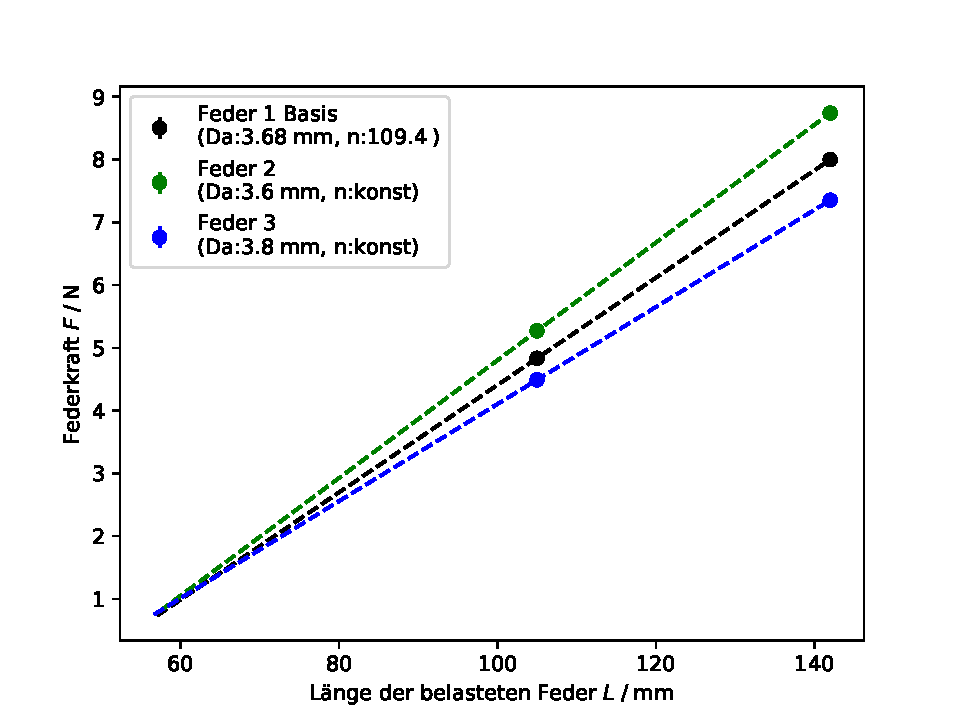
\includegraphics{build/D_kraftweg_dia.pdf}
    \caption{Feder 1,2,3 mit unterschiedlichen Federdurchmessern $D$.
    Aufgetragen in einem Kraft-Weg-Diagramm. Gemessen wurden dabei
    die für L1 und L2 resultierenden Federkräfte F1 und F2.}
\end{figure}

\begin{figure}
    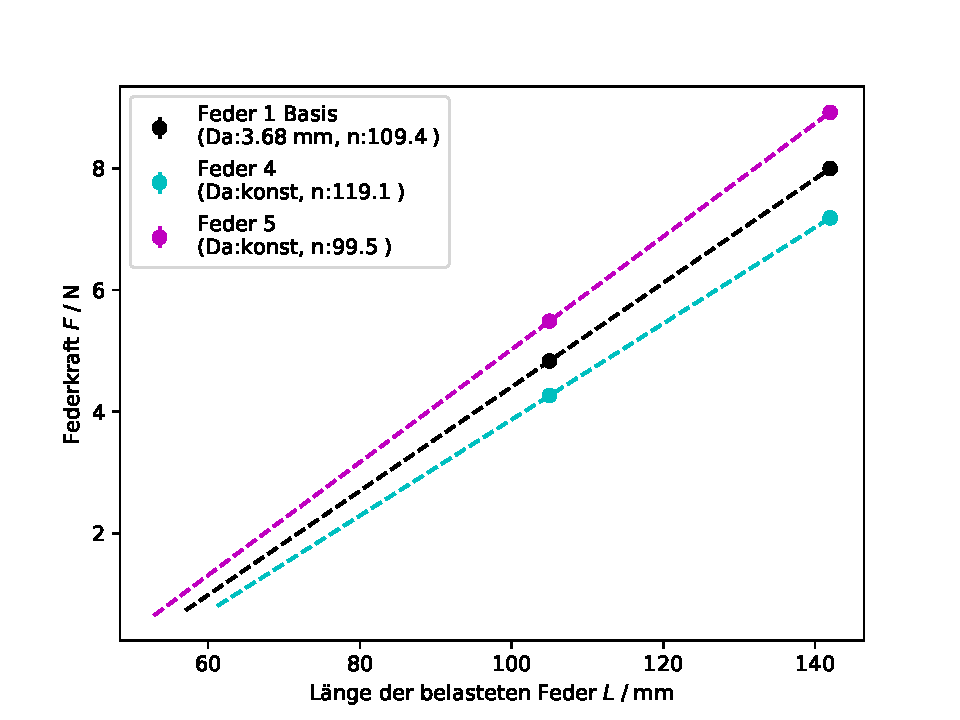
\includegraphics{build/n_kraftweg_dia.pdf}
    \caption{Feder 1,4,5 mit unterschiedlichen Windungszahlen $n$.
    Aufgetragen in einem Kraft-Weg-Diagramm. Gemessen wurden dabei die für L1
    und L2 resultierenden Federkräfte F1 und F2}
\end{figure}


\label{sec:Auswertung}
